\chapter{Grundlagen}
\thispagestyle{standard}
\pagestyle{standard}
\renewcommand{\footrulewidth}{0.4pt}
\lfoot{\small Refik Kerimi}

Wie in Kapitel \ref{chap:Einleitung} beschrieben, hat der stetige Zuwachs von \acs{PWA}s zum Umdenken bei der Planung und beim Entwickeln von Webapplikationen geführt \cite{DERs}.
Diese Arbeit beschäftigt sich mit der Frage "Können Progressive Web Apps Native Apps zur Gänze ersetzten?".
 


\begin{figure}[h]
	\centering
	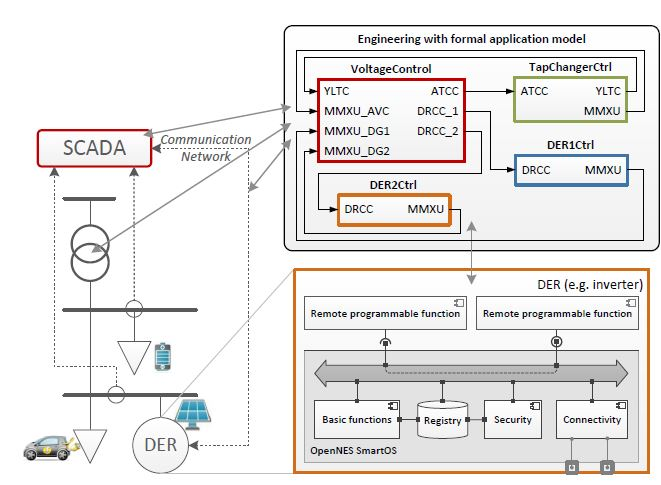
\includegraphics[width=14cm]{BilderAllgemein/OpenNES_architecture}\medskip
	\caption{Übersicht des OpenNES Konzepts \cite{OpenNES}}
	\label{fig:Übersicht des OpenNES Konzepts}
\end{figure}

 
\section{Geschichte Applikationsentwicklung}

\begin{itemize}
    \item Das Betriebssystem mit den Basis- und Kommunikationsfunktionen
	\item Das Sicherheitsmodul und austauschbare \ac{SWK}
	\item Die Entwicklungsumgebung um die \acs{SWK} zu programmieren oder neu zu konfigurieren
\end{itemize}



\newpage
\section{Mobile APP}


\subsection{Native Apps}





\subsection{Webapplikationen}


\subsection{Progressive Web Apps}


\subsection{Unterschiede zwischen Web Apps PWA und Native Apps}

\newpage























